\chapter{Branching}
\section{Begriffserklärung}
Bei einem Commit speichert Git ein Commit-Objekt ab. Dieses Objekt enthält einen Zeiger auf den Snapshot mit den Objekten der Staging Area, Autor, Metadaten und einen Zeiger auf die direkten Eltern-Commits. Projektverzeichnisse werden als tree-Objekt abgelegt und Projektdateien als Blob gespeichert.
\begin{figure}[htb]
    \centering
    \begin{minipage}[t]{0.48\linewidth}
        \centering
        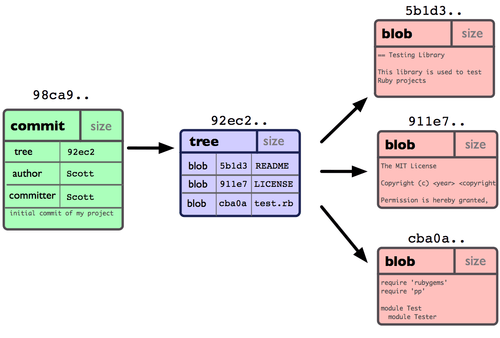
\includegraphics[width=\linewidth]{img/tree.png}
        \caption{Commit Daten}
    \end{minipage}% <- sonst wird hier ein Leerzeichen eingefügt
    \hfill
    \begin{minipage}[t]{0.48\linewidth}
        \centering
        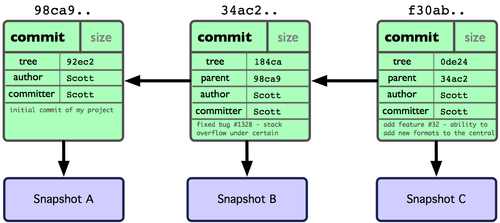
\includegraphics[width=\linewidth]{img/commits.png}
        \caption{mehrere Commits}
    \end{minipage}
\end{figure}
Ein Branch in Git ist ein Zeiger auf einen dieser Commits. Der Standard Git Branch heißt \texttt{master}. Dieser wird mit dem Initial Commit erstellt. Beim Erstellen eines neuen Branches wird ein neuer Zeiger erstellt. Dieser zeigt auf den gleichen Commit, auf welchem gerade gearbeitet wird. Dies wird über den HEAD-Zeiger realisisert, welcher auf den aktullen lokalen Branch zeigt.
\begin{figure}[ht]
	\centering
		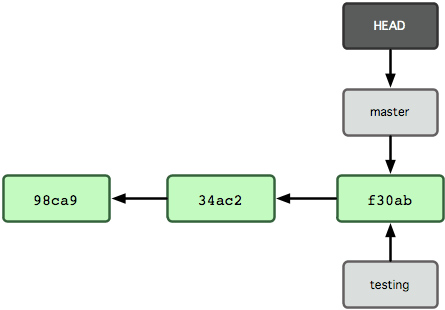
\includegraphics[width=0.6\textwidth]{img/branch.png}
	\caption{Branch erstellen}
\end{figure}
\newpage
\section{Branch anlegen}
\begin{lstlisting}[caption={Branch anlegen},captionpos=b]
#create branch
git branch [branchname]

#create branch, activate and switch to it
git checkout -b [branchname]
\end{lstlisting}
\section{Branch wechseln}
\begin{lstlisting}[caption={Branch wechseln},captionpos=b]
git checkout [branchname]
\end{lstlisting}
\section{Arbeiten mit Branches}
Auf jeden Branch kann unabhängig zu anderen Branches gearbeitet werden. Beim Wechseln des Branches wird lediglich der HEAD Zeiger verschoben und alle Dateien im Arbeitsverzeichnis auf den Stand des letzten Commits des Branches in den gewechselt wird versetzt. Commitete Änderungen des anderen Branches bleiben natürlich erhalten. Da Branches selbst keinerlei Dateien enthalten und nur aus einer kleinen Datei bestehen (SHA-1 Prüfsumme), können diese einfach erstellt und entfernt werden.
\begin{figure}[ht]
	\centering
		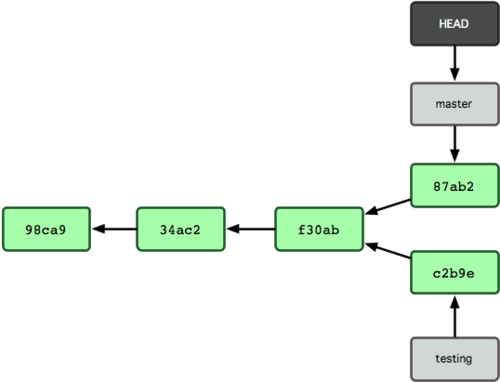
\includegraphics[width=0.8\textwidth]{img/branches.png}
	\caption{Verzweigte Branches}
\end{figure}
\newpage
\section{Einfaches Branching und Merging}
Änderungen, Verbesserung, etc. sollten nicht im Produktivzweig erstellt werden. Hierzu ist es ratsam einen extra Branch für die Entwicklung zu erstellen. Hierzu ein einfaches Beispiel anhand einer Webentwicklung:
\begin{lstlisting}[caption={Einfaches Merging Beispiel},captionpos=b]
#Branch erstellen
git branch dev

#Branch wechseln
git checkout dev

#Entwicklung
vim index.html

#Commit
git commit -a -m 'Content added'

#Zum Master Branch wechseln und zusammenfuehren von Master und Dev
git checkout master
git merge dev

#Entwicklungsbranch entfernen
git branch -d dev
\end{lstlisting}
\section{Grundlagen des Zusammenführens (Merge)}
\begin{center}
\renewcommand{\arraystretch}{1.2}
\begin{tabular}{|p{4cm}p{10cm}|}
\hline
\textbf{Vorgehen}			&\textbf{Beschreibung}\\
\hline
\texttt{fast forward}			&Neuer Commit direkter Nachfolger von ursprünglichen Commit. Einfaches Merging. Zeiger wird einfach auf neuen Commit weiter bewegt (kein neuer Commit).\\
\hline
\texttt{recursive strategy}		&Kein direkter Nachfolger. 3-Wege-Merge. Neuer Commit wird angelegt. Git ermittelt selbstständig die besten 3 Eltern (merge commit).\\
\hline
\end{tabular}
\captionof{table}{Merge Strategien}
\renewcommand{\arraystretch}{1}
\end{center}
\section{Merge Konflikte}
Wurden an den selben Stellen in den selben Dateien unterschiedlicher Branches etwas geändert, können diese Änderungen von Git nicht sauber zusammengefügt werden. Dies führt zu einen Merge Conflict. Diese Dateien werden als \texttt{unmerged} aufgelistet und mit Markern versehen um die Konflikte manuell zu lösen. Nach dem Auflösen des Konflikts müssen die Dateien per \texttt{git add} der Staging Area hinzugefügt werden. Das Staging markiert sie für Git als gereinigt. Anschließend nochmals mit \texttt{git status} überprüfen, ob alle Konflikte aufgelöst wurden und den Merge mit \texttt{git commit} abschießen.
\section{Branch Management}
\begin{lstlisting}[caption={Branch Management},captionpos=b]
# list branches
git branch

#last commit per branch
git branch -v

#display only merged branches
git branch --merged

#display only unmerged branches
git branch --unmerged

#branches with unmerged changes
git branch --no-merged

#delete branch with unmerged changes
git branch -D [branchname]
\end{lstlisting}
\section{Workflows}
\subsection{Langfristige Branches}
Master Branch mit stabilen Code. Entwicklung in seperaten Branch (bzw. auch mehrere Branches möglich). Nur stabiler Code wird in den Master Branch gemerged.
\begin{figure}[ht]
	\centering
		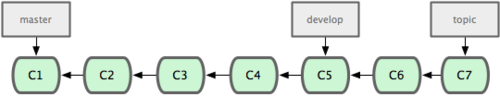
\includegraphics[width=0.5\textwidth]{img/longterm.png}
	\caption{Langfristige Brances}
\end{figure}
\subsection{Themen Branches}
Kurzlebige Zweige für die Entwicklung spezieller Features und Funktionen. Diese Branches liegen nur lokal vor.
\begin{figure}[ht]
	\centering
		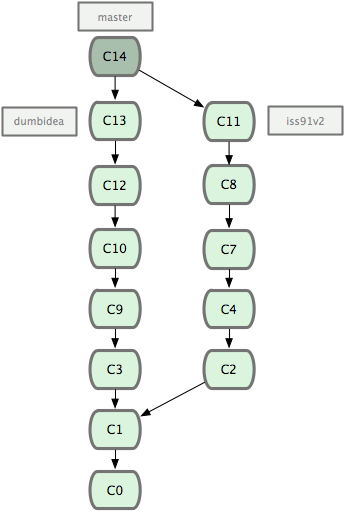
\includegraphics[width=0.22\textwidth, angle=90]{img/thema.png}
	\caption{Themen Branches}
\end{figure}
\section{Externe Branches}
\section{Rebasing}
In Git gibt es zwei Methoden Änderungen in einen anderen Branch zu überführen. Neben dem \texttt{merge} existiert das \texttt{rebase} Kommando.
\subsection{einfaches Rebase}
Bei einem einfachen Rebase wird der Vorfahr eines Zweiges geändert. Dies dient dazu einen 3-Wege-Merge zu vermeiden, sodass ein einfacher Fast-Forward-Merge durchgeführt werden kann.
\begin{lstlisting}[caption={Einfaches Rebase},captionpos=b]
#Branch to rebase
git checkout dev

#Rebase Branch
git rebase master

#Change to Master and merge
git checkout master
git merge dev

#Rebase without Checkout
rebase [Basis-Branch] [Themen-Branch]
\end{lstlisting}
\subsection{Rebasing auf anderen Branch}
\begin{lstlisting}[caption={Rebase auf anderen Branch},captionpos=b]
git rebase --onto master server client
\end{lstlisting}
\begin{figure}[ht]
	\centering
		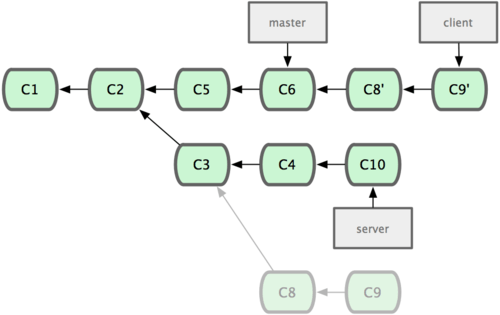
\includegraphics[width=0.6\textwidth]{img/rebase.png}
	\caption{Themen Branches}
\end{figure}
\textbf{Rebase keine Commits die in ein öffentliches Repository hochgeladen wurden}

